% !TeX spellcheck = en_GB
\begin{figure}[t]
	\centering
%%%%%% 20/12
    \begin{subfigure}[b]{0.49\textwidth}
        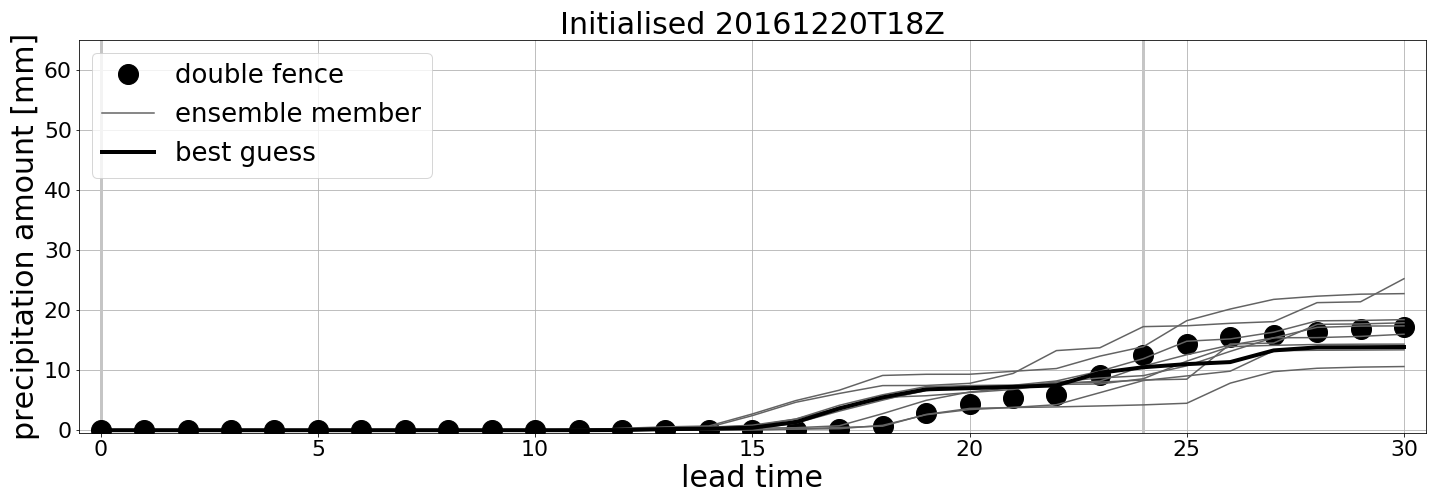
\includegraphics[
        width=\textwidth]{./fig_MEPS_sfc/20161220_18}
        \caption{}\label{fig:acc20}
        %\label{fig:DT2100}
    \end{subfigure}
    \hfill
%%%%%% 21/12
    \begin{subfigure}[b]{0.49\textwidth}
        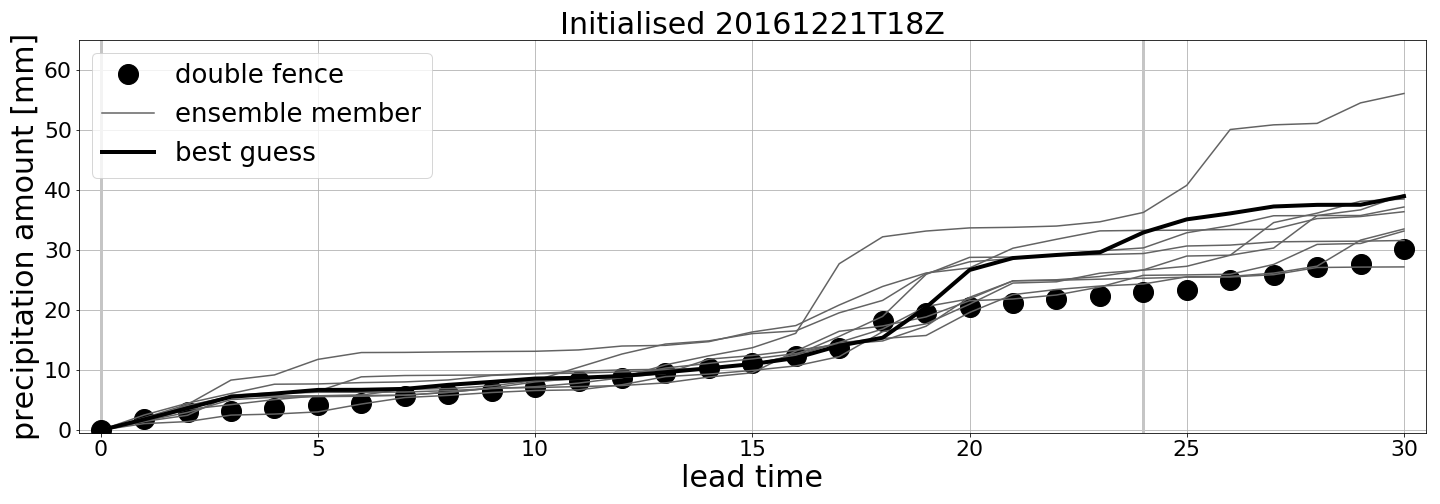
\includegraphics[
        width=\textwidth]{./fig_MEPS_sfc/20161221_18}
        \caption{}\label{fig:acc21}
    \end{subfigure}
%%%%%% 22/12
    \begin{subfigure}[b]{0.49\textwidth}
        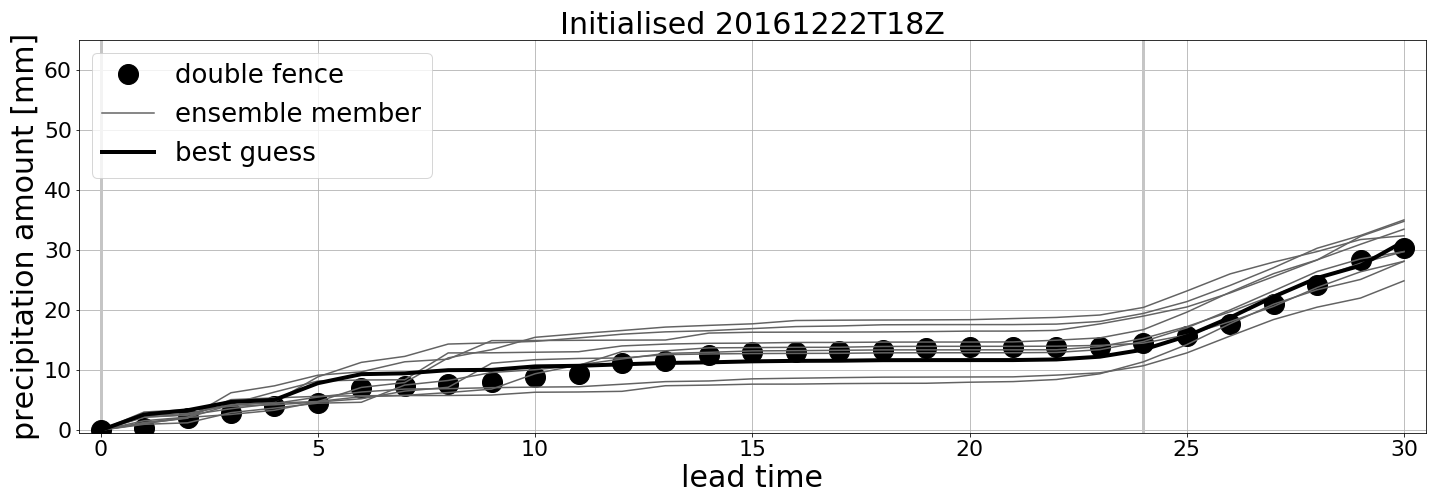
\includegraphics[
        width=\textwidth]{./fig_MEPS_sfc/20161222_18}
        \caption{}\label{fig:acc22}
    \end{subfigure}
    \hfill
%%%%%% 23/12
    \begin{subfigure}[b]{0.49\textwidth}
        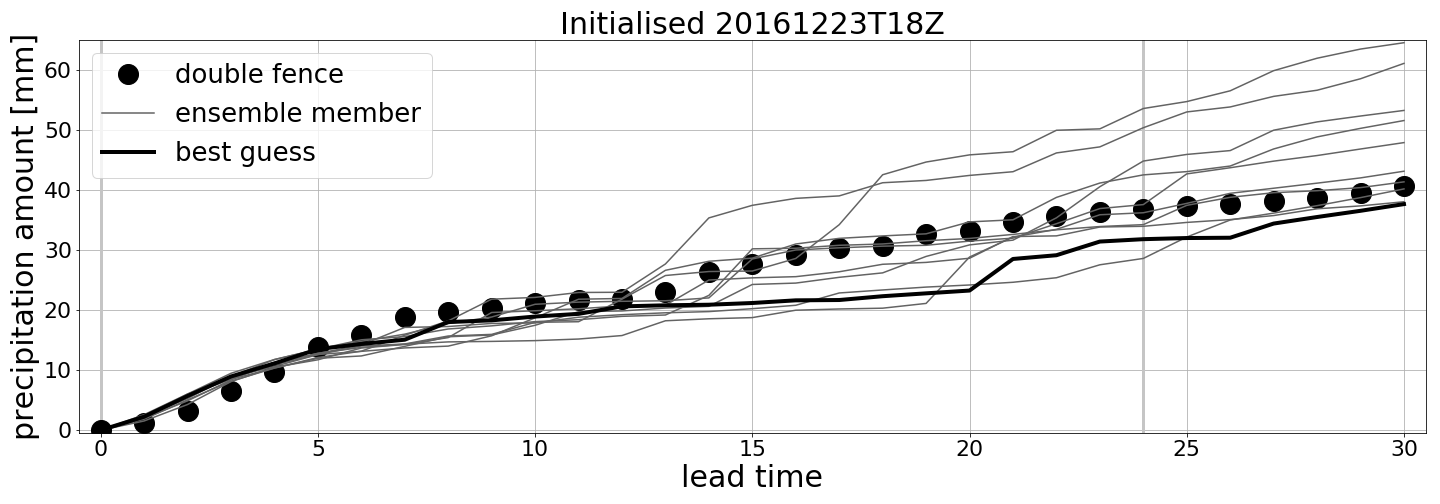
\includegraphics[
        width=\textwidth]{./fig_MEPS_sfc/20161223_18}
        \caption{}\label{fig:acc23}
    \end{subfigure}
%%%%%% 24/12
    \begin{subfigure}[b]{0.49\textwidth}
        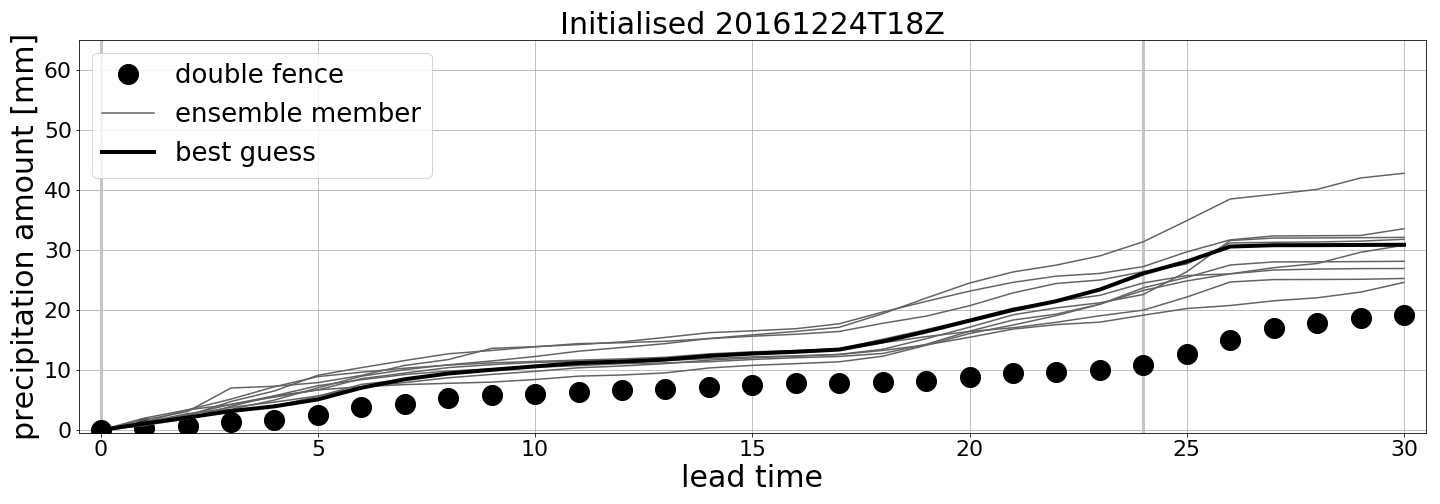
\includegraphics[
        width=\textwidth]{./fig_MEPS_sfc/20161224_18}
        \caption{}\label{fig:acc24}
    \end{subfigure}
    \hfill
%%%%%% 25/12
    \begin{subfigure}[b]{0.49\textwidth}
        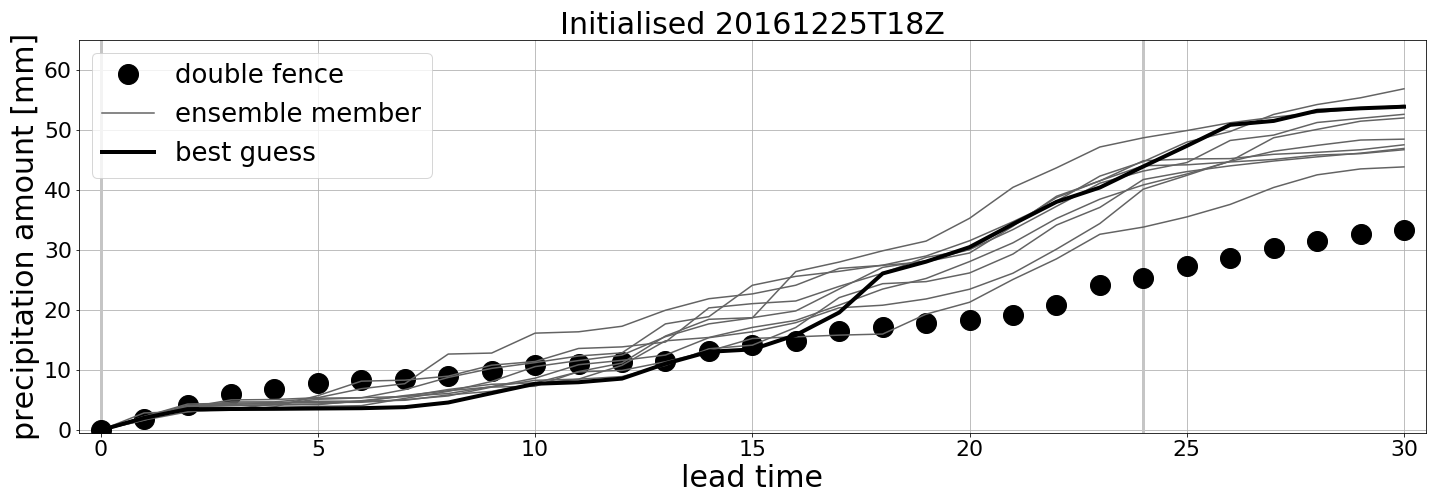
\includegraphics[
        width=\textwidth]{./fig_MEPS_sfc/20161225_18}
        \caption{}\label{fig:acc25}
    \end{subfigure}
    \caption{Accumulation of precipitation at Haukeliseter. Initalisation of MEPS at \SI{18}{\UTC}. Ensemble member as line in grey and the control in black. Dots indicate the hourly accumulation observed at the double fence, \citep{eklima_norwegian_2016}. \textcolor{red}{Do you think I have to make something bigger??? Font size etc? Or use one page only for the figures and have them underneath each other?} } \label{fig:acc20_25}
\end{figure}